%Chapter 3

\renewcommand{\thechapter}{3}

\chapter{Hierarchical Consensus}
\label{ch:hierarchical_consensus}
% Overview, details, consistency, performance, lessons learned.

% This paragraph sucks.
The backbone of our planetary scale data system is \emph{hierarchical consensus}~\cite{hc_brief_announcement}.
Hierarchical consensus provides a strong consistency foundation that totally orders critical accesses and arbitrates the eventual consistency layer in the fog, which raises the overall consistency of the system.
To be effective, an externalizable view of consistency ordering must be available to the entire system.
This means that strong consistency must be provided across geographic links rather than provided as localized, independent decision making with periodic synchronization.
The problem that hierarchical consensus is therefore designed to solve is that of distributed consensus.

Solutions to distributed consensus primarily focus on providing high throughput, low latency, fault tolerance, and durability.
Current approaches \cite{epaxos,mencius,calvindb,spaxos,sutra_fast_2011,peluso_making_2016} usually assume a small number of replicas, each centrally located on a highly available, powerful, and reliable host.
These assumptions are justified by the environments in which they run: highly curated environments of individual data centers connected by dedicated networks.
Although replicas in these environments may participate in global consensus, our data model requires us to accommodate replicas with heterogenous capabilities and usage modalities.
Widely distributed replicas might have neither high bandwidth nor low latency and might suffer partitions of varying durations.
Such systems of replicas might also be dynamic in membership, in relative locations, and have relative workloads.
Most importantly, to provide a backbone for a planetary scale data system, the consistency backbone must scale to include potentially hundreds of replicas around the world.

As a result, straightforward approaches of running variants of Paxos~\cite{paxos}, ePaxos~\cite{epaxos}, or Raft~\cite{raft} across the wide area, even for individual objects will perform poorly for several reasons.
First, distance (in network connectivity) between consensus replicas and the most active replicas decrease the performance of the entire system, consensus is only as fast as the final vote required to make a decision, even when making thrifty requests.
Second, network partitions are common, which cause consensus algorithms to fail-stop~\cite{fail-stop} if they cannot receive a majority, a criticism that is often used to justify eventual consistency systems for high availability.
Finally, the fault tolerance of small quorum algorithms can be disrupted by a small number of unreliable hosts and given the scale of the system and the heterogenous nature of replicas, the likelihood of individual failure is so high so as to be considered inevitable.

% what about spanner, mdcc, and calvin?

We propose another approach to building large systems.
Rather than relying on a few replicas to provide consensus to many clients, we propose to run a consensus protocol across replicas running at or near all of these locations.
The key insight is that large problem spaces can often be partitioned into mostly disjoint sets of activity without violating consistency.
We exploit this decomposition property by making our consensus protocol hierarchical and individual consensus groups fast by ensuring they are small.
We exploit locality by building subquorums from colocated replicas, and locating subquorums near clients they serve.

In this chapter we describe hierarchical consensus, a two-tiered consensus structure that allows high throughput, localization, agility, and linearizable access to a shared namespace. We show how to use \emph{delegation} to build large consensus groups that retain their fault tolerance properties while performing like small groups. We describe the use of \emph{fuzzy epoch transitions} to allow global re-configurations across multiple consensus groups without forcing them into lockstep. Finally, we describe how we reason about consistency by describing the structure of grid consistency.

\section{Overview}

Hierarchical Consensus (HC) is an implementation and extension of Vertical Paxos~\cite{vertical_paxos,boxwood,niobe} designed to scale to hundreds of nodes geo-replicated around the world.
Vertical Paxos divides consensus decisions both horizontally, as sequences of consensus instances, and vertically as individual consensus decisions are made.
Spanner~\cite{spanner}, MDCC~\cite{mdcc}, and Calvin~\cite{calvindb}, can all be thought of as implementations of Vertical Paxos, in that they shard the namespace of the objects they manage into individual consensus groups (the vertical division).
In these cases, however, sharding does not allow for inter-object dependence (the horizontal division) without either a management quorum which is either not geo-replicated, suffers from the same problems in scaling, or without the use of extremely accurate timestamps.
The challenge is therefore in building a multi-group coordination protocol that configures and mediates the subquorums with the same level of consistency and fault tolerance of the entire system.

\begin{figure}
    \begin{center}
        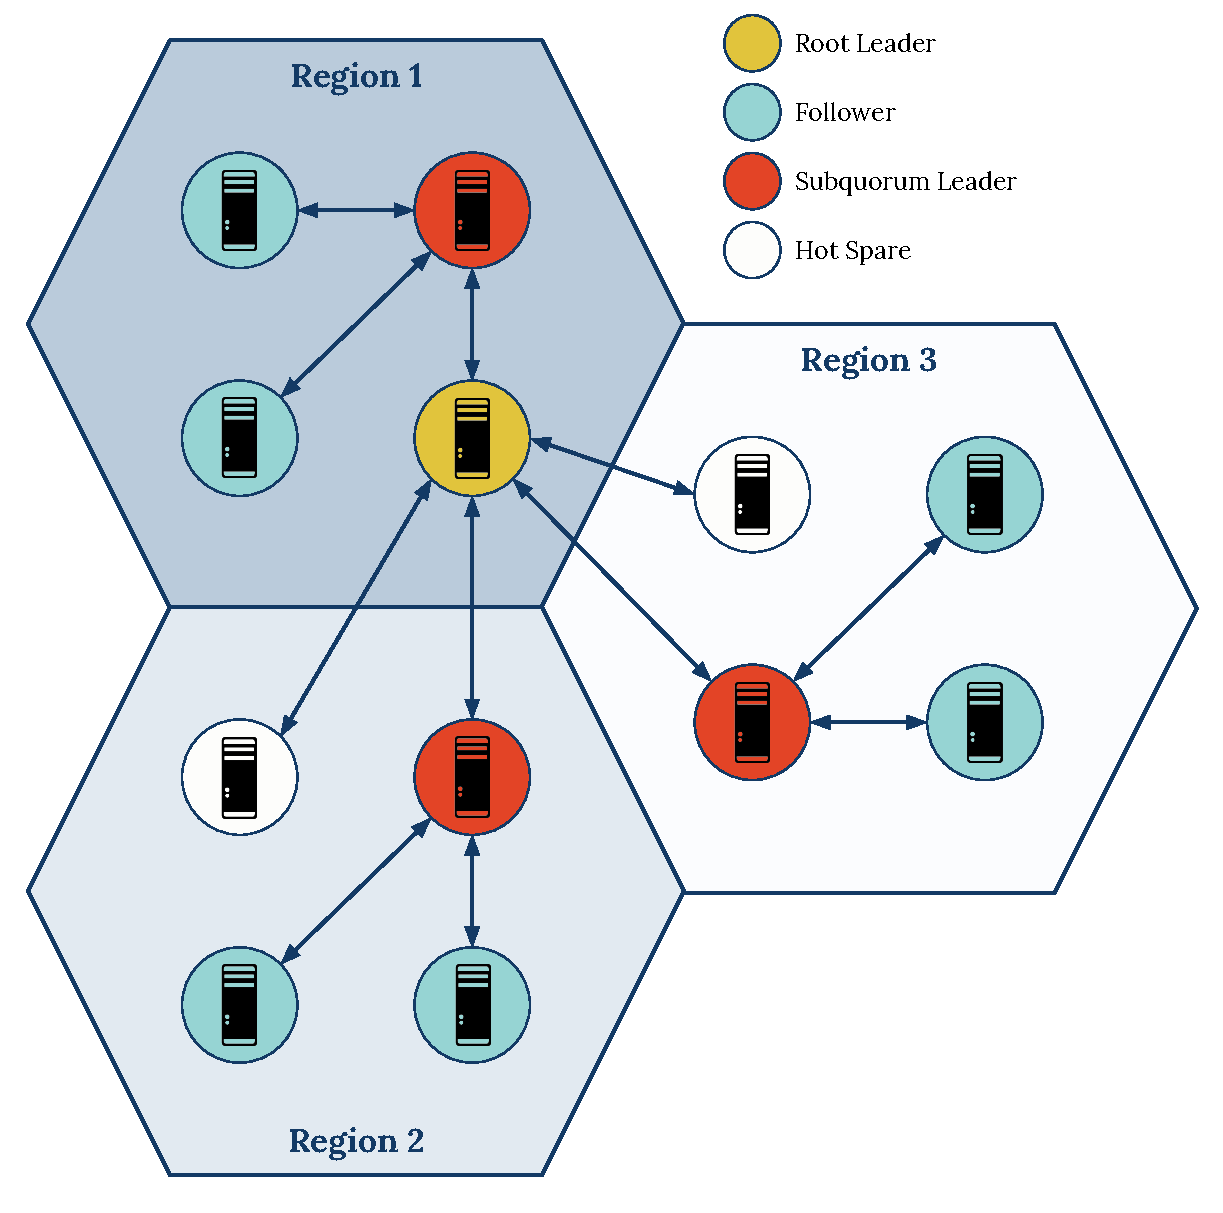
\includegraphics[width=5in]{figures/ch03_hierarchical_topology.pdf}
    \end{center}
    \renewcommand{\baselinestretch}{1}
    \small\normalsize

    \begin{quote}
        \caption[A 12x3 Hierarchical Consensus Network Topology]{A simple example of an HC network composed of 12 replicas with size 3 subquorums. Each region hosts its own subquorum and subquorum leader, while the subquorum leaders delegate their votes to the root quorum, whose leader is found in region 1. This system also has 2 hot spares that can be used to quickly reconfigure subquorums that experience failures. The hot spares can either delegate their vote, or participate directly in the root quorum.}
        \label{fig:ch03_hierarchical_topology}
    \end{quote}
\end{figure}
\renewcommand{\baselinestretch}{2}
\small\normalsize

Hierarchical consensus therefore organizes \emph{all} participating replicas to participate in a root quorum as shown in Figure~\ref{fig:ch03_hierarchical_topology}.
The root quorum guarantees correctness by pivoting the overall system through two primary functions.
First, the root quorum reconfigures subquorum memberships on replica failures and system membership changes (allocating hot-spares as needed).
Second, the root quorum adjusts the mapping of the object namespace to the underlying partitions.
Much of the system's complexity comes from handshaking between the root quorum and the lower-level subquorums during reconfigurations.

These handshakes are made easier, and much more efficient, by using \emph{fuzzy transitions}.
Fuzzy transitions allow individual subquorum to move through reconfiguration at their own pace, allowing portions of the system to transition to decisions made by the root quorum before others.
Given out heterogenous, wide-area environment, forcing the entire system to transition to new configurations in lockstep would be unacceptably slow.
Fuzzy transitions also ensure that there is no dedicated shard-master that has to synchronize all namespace allocations: at the cost of possibly multiple  redirections, clients can be redirected by any member of the root quorum to replicas who should be participating in consensus decisions for the requested objects.

Fuzzy transitions ensure that root quorum decisions need not be timely since those decisions do not disrupt accesses of clients.
Though root quorum decisions are rare with respect to the throughput of accesses inside the entire system, they still do require the participation of all members of the system, which could lead to extremely large quorum sizes, and therefore extremely slow consensus operations that may be extremely sensitive to partitions.
Because all subquorums make disjoint decisions and because all members of the system are part of the root quorum, we propose a safe relaxation of the participation requirements for the root quorum such that subquorum followers can \emph{delegate} their root quorum votes to their leader.
Delegation ensures that only a small number of replicas participate in most root quorum decisions, though decisions are made for the entire system.

In brief, the resulting system is local, in that replicas serving clients can be located near them.
The system is fast because individual operations are served by small groups of replicas, regardless of the total size of the system.
The system is nimble in that it can dynamically reconfigure the number, membership, and responsibilities of subquorums in response to failures, phase changes in the driving applications, or mobility among the member replicas.
Finally, the system is consistent, supporting the strongest form of per-object consistency without relying on special-purpose hardware~\cite{fawn,corfu,vcorfu,tango,spanner}.

\begin{figure}
    \begin{center}
        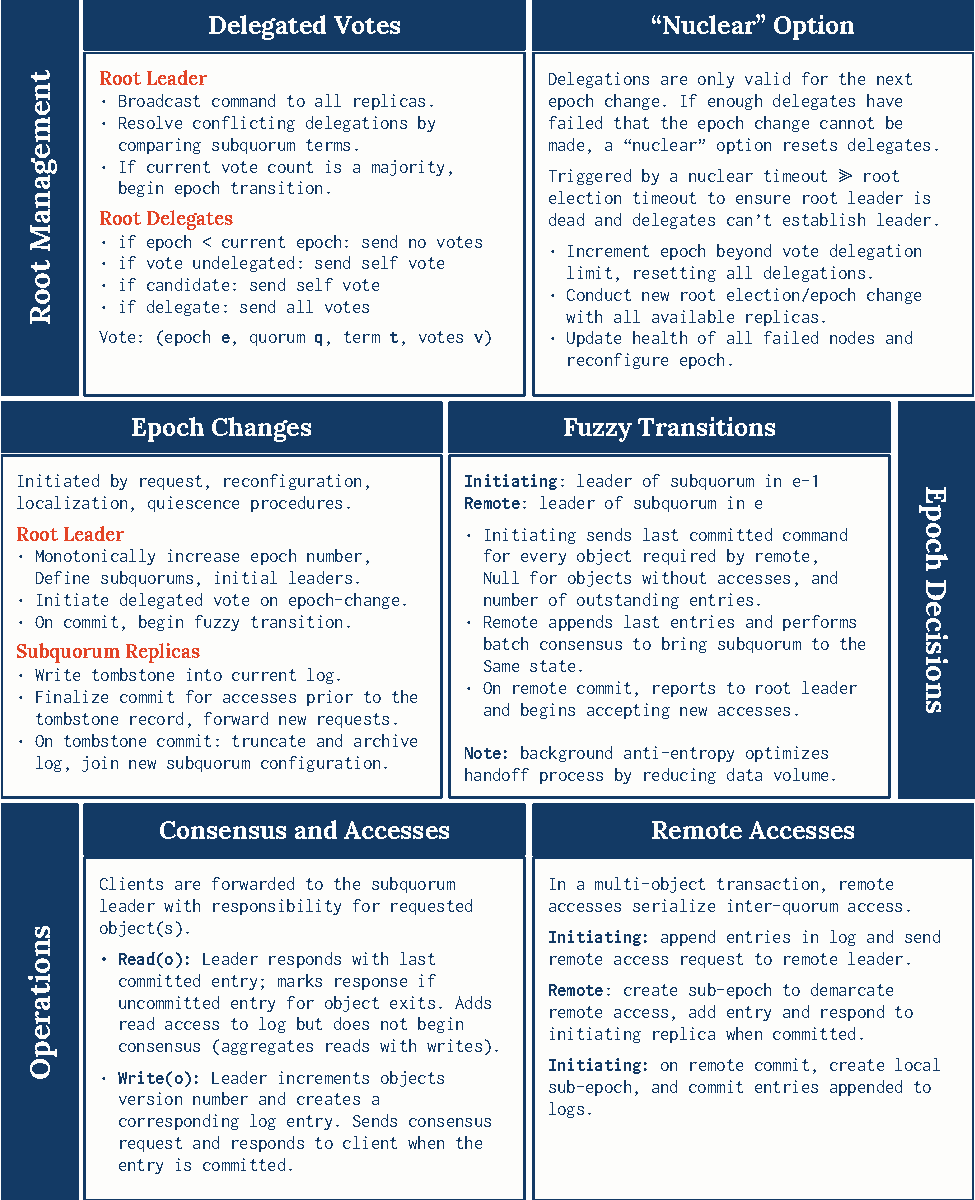
\includegraphics[width=5in]{figures/ch03_hc_operation_summary.pdf}
    \end{center}
    \renewcommand{\baselinestretch}{1}
    \small\normalsize

    \begin{quote}
        \caption[HC Operational Summary]{A condensed summary of the hierarchical consensus protocol. Operations are described in a top-to-bottom fashion where the top level is root quorum operations, the bottom is subquorum operations, and the middle is transition and intersection.}
        % Section numbers such as §5.2 indicate where particular features are discussed.
        \label{fig:ch03_hc_operation_summary}
    \end{quote}
\end{figure}
\renewcommand{\baselinestretch}{2}
\small\normalsize

A complete summary of hierarchical consensus is described in Figure~\ref{fig:ch03_hc_operation_summary}.

\section{Consensus}

The canonical distributed consensus used by systems today is Paxos~\cite{paxos,paxos_simple}.
Paxos is provably safe and designed to make progress even when a portion of the system fails.
Raft~\cite{raft} was designed not to improve performance, but to increase understanding of consensus behavior to better allow efficient implementations.
HC uses Raft as a building block, so we describe the relevant portions of Raft at a high level, referring the reader to the original paper for complete details.
Though we chose to base our protocol on Raft, a similar approach could be used to modify Paxos into a hierarchical structure.

Consensus protocols typically have two phases: leader \emph{election} and operations \emph{commit}\renewcommand{\baselinestretch}{1} \small\footnotesize\footnote{Election and commit phases correspond to PROPOSE and ACCEPT phases in Paxos}\renewcommand{\baselinestretch}{2} \small\normalsize.
Raft is a strong-leader consensus protocol, which allows the election phase to be elided while a leader remains available.
The protocol requires only a single communication round to commit an operation in the common case.
Raft uses timeouts to trigger phase changes and provide fault tolerance.
Crucially, it relies on timeouts only to provide progress, not safety.
New elections occur when another replica in the quorum times out waiting for communication from the leader.
Such a replica increments its \emph{term} until it is greater than the existing leader, and announce its candidacy.
Other replicas vote for the candidate if they have not seen a competing candidate with a larger term.
During regular operation, clients send requests to the leader, which broadcasts \texttt{AppendEntries} messages carrying operations to all replicas.
An operation is \emph{committed} and can be executed when the leader receives acknowledgments of the \texttt{AppendEntries} message from more than half the replicas (including itself).

\todo{We describe differences in our Raft implementation from the canonical implementation in Chapter~\ref{ch:system_implementation}}

Throughout the rest of this chapter we use the term \emph{root quorum} to refer to the upper, namespace-mapping and configuration-management tier of HC, and \emph{subquorum} to describe a group of replicas (called \emph{peers}) participating in consensus decisions for a section of the namespace.
The root quorum shepherds subquorums through \emph{epochs}, each with potentially different mappings of the namespace and replicas to subquorums.
An epoch corresponds to a single commit phase of the root quorum.
We use the term Raft only when describing details particular to our current use of Raft as the underlying consensus algorithm.
We refer to the two phases of the base consensus protocol as the \emph{election phase} and the \emph{commit phase}.
We use the term \emph{vote} as a general term to describe positive responses in either phase.
Epoch $x$ is denoted $e_x$.
Subquorum $i$ of epoch $e_x$ is represented as $q_{i,x}$, or just $q_i$ when the epoch is obvious.
$t_a$ represents a specific \emph{tag}, or disjoint subset of the namespace.

We assume faults are fail-stop~\cite{fail-stop} rather than Byzantine~\cite{byzantine-generals}.
We do not assume that either replica hosts or networks are homogeneous, nor do we assume freedom from partitions and other network faults.


\subsection{Root Consensus}

\begin{figure}
    \begin{center}
        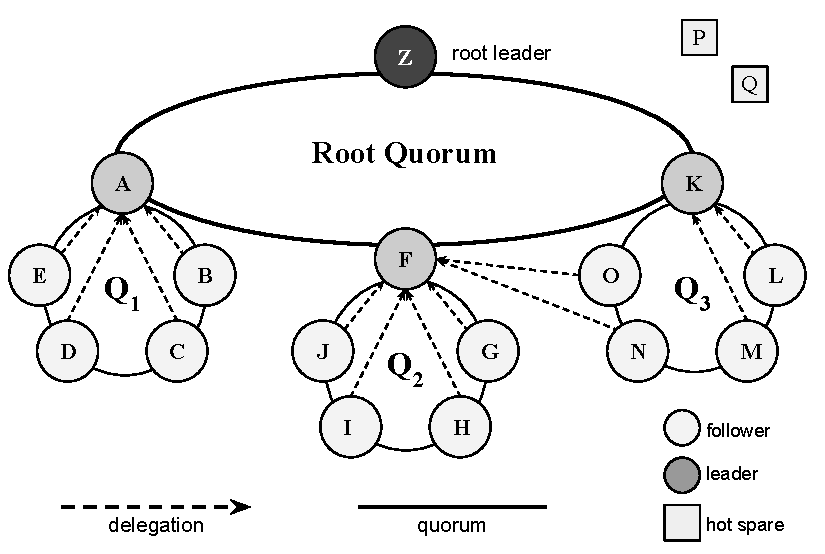
\includegraphics[width=5in]{figures/ch03_election.pdf}
    \end{center}
    \renewcommand{\baselinestretch}{1}
    \small\normalsize

    \begin{quote}
        \caption[Delegated Votes]{}
        \label{fig:ch03_tiers}
    \end{quote}
\end{figure}
\renewcommand{\baselinestretch}{2}
\small\normalsize

Hierarchical consensus is a leader-oriented protocol that organizes replicas into two tiers of quorums, each responsible for fundamentally different decisions (Figure~\ref{fig:ch03_tiers}).
The lower tier consists of multiple independent subquorums, each committing operations to local shared logs.
The upper,  \emph{root quorum}, consists of subquorum peers, usually their leaders, delegated to represent the subquorum in root elections and commits.
Hierarchical consensus's main function is to export a linearizable abstraction of shared accesses to some underlying substrate, such as a distributed object store or file system.
We assume that nodes hosting object stores, applications, and HC are frequently co-located across the wide area.

The root quorum's primary responsibilities are mapping namespaces and replicas to individual subquorums.
Each such map defines a distinct epoch, $e_i$, a monotonically increasing representation of the term of $q_{i,e}$.
The root quorum is effectively a consensus group consisting of subquorum leaders.
Somewhat like subquorums, the effective membership of the root quorum is not defined by the quorum itself, but in this case by leader election or peer delegations in the lower tier.

The root quorum partitions the namespace across multiple subquorums, each with a disjoint portion as its scope.
The intent of subquorum localization is ensure that the \emph{domain} of a client, the portion of the namespace it accesses, is entirely within the scope of a local, or nearby, subquorum.
If true across the entire system, each client interacts with only one subquorum, and subquorums do not interact at all during execution of a single epoch.
This \emph{siloing} of client accesses simplifies implementation of strong consistency guarantees and allows better performance.

\subsection{Delegation}

Fault tolerance scales with increasing system size.
The root quorum's membership is, at least logically, the set of all system replicas, at all times.
However, running consensus elections across large systems is inefficient in the best of cases, and prohibitively slow in a geo-replicated environment.
Root quorum decision-making is kept tractable by having replicas \emph{delegate} their votes, usually to their leaders, for a finite duration.
With leader delegation, the root membership effectively consists of the set of subquorum leaders.
Each leader votes with a count describing its own and peer votes from its
subquorum.

Consider an alternative leader-based approach where root quorum membership is defined as the current set of subquorum leaders.
Both delegation and the leader approach have clear advantages in performance and flexibility over direct votes of the entire system.
However, the leader approach dramatically decreases fault tolerance.
Furthermore, the root quorum becomes unstable in the leader approach as its membership changes during partitions or subquorum elections.
% Furthermore, \roo membership changes with \sub leaders and at \sub
% repartitions in the leader approach.
These changes would require heavyweight \emph{joint consensus} decisions in the root quorum for correctness in Raft-like protocols~\cite{raft}.

With delegation, however, root quorum membership is always the entire system and remains unchanged over subquorum re-configuration.
Delegation is essentially a way to optimistically shortcut contacting every replica for each decision.
Subquorum repartitioning merely implies that a given replica's vote might need to be delegated to a different leader.

Delegation does add one complication: the root quorum leader must know all vote delegations to request votes when committing epoch changes.
We deal with this issue, as well as the requirement for a nuclear option (Section~\ref{sec:nuclear}), by simplifying our protocol.
Instead of sending vote requests just to subquorum leaders, \textbf{the root quorum leader sends vote requests to all system replicas.}
This is true even for \emph{hot spares}, which are not currently in any subquorum.

This is correct because vote requests now reach all replicas, and because replicas whose votes have been delegated merely ignore the request.
We argue that it is also efficient, as a commit's efficiency depends only on receipt of a majority of the votes.
Large consensus groups are generally slow (see Section~\ref{sec:evaluation}) not just because of communication latency, but because large groups in a heterogeneous setting are more likely to include replicas on very slow hosts or networks.
In the usual case for our protocol, the root leader still only needs to wait for votes from the subquorum leaders.
Leaders are generally those that respond more quickly to timeouts, so the
speed of root quorum operations is unchanged.
% Not generally true, as timeouts are stochastic.

\subsection{Epoch Transitions}

% - tagspace (prefix-trie)
% - fuzzy transitions
% - anti-entropy and tombstones

An epoch change is initiated by the leader in response to one of several events, including:

\renewcommand{\baselinestretch}{1}
\begin{itemize}
    \item a namespace repartition request from a subquorum leader
    \item notification of join requests by new replicas
    \item notification of failed replicas
    \item changing network conditions that suggest re-assignment of replicas
\end{itemize}
\renewcommand{\baselinestretch}{2}

The root leader transitions to a new epoch through the normal commit phase in the root quorum.
The command proposed by the leader is an enumeration of the new subquorum partition, namespace partition, and assignment of namespace portions to specific subquorums.
The announcement may also include initial leaders for each subquorum, with the usual rules for leader election applying otherwise, or if the assigned leader is unresponsive.
Upon commit, the operation serves as an \emph{announcement} to subquorum leaders.
Subquorum leaders repeat the announcement locally, disseminating full knowledge of the new system configuration, and eventually transition to the new epoch by committing an \texttt{epoch-change} operation locally.

The epoch change is lightweight for subquorums that are not directly affected by the underlying re-configuration.
If a subquorum is being changed or dissolved, however, the \emph{epoch-change} commitment becomes a tombstone written to the logs of all local replicas.
No further operations will be committed by that version of the subgroup, and the local shared log is archived and then truncated.
Truncation is necessary to guarantee a consistent view of the log within a subquorum, as peers may have been part of different subquorums, and thus have different logs, during the last epoch.
Replicas then begin participating in their new subquorum instantiation.
In the common case where a subquorum's membership remains unchanged across the transition, an \texttt{epoch-change} may still require additional mechanism because of changes in namespace responsibility.

\begin{landscape}
\begin{figure}
    \begin{center}
        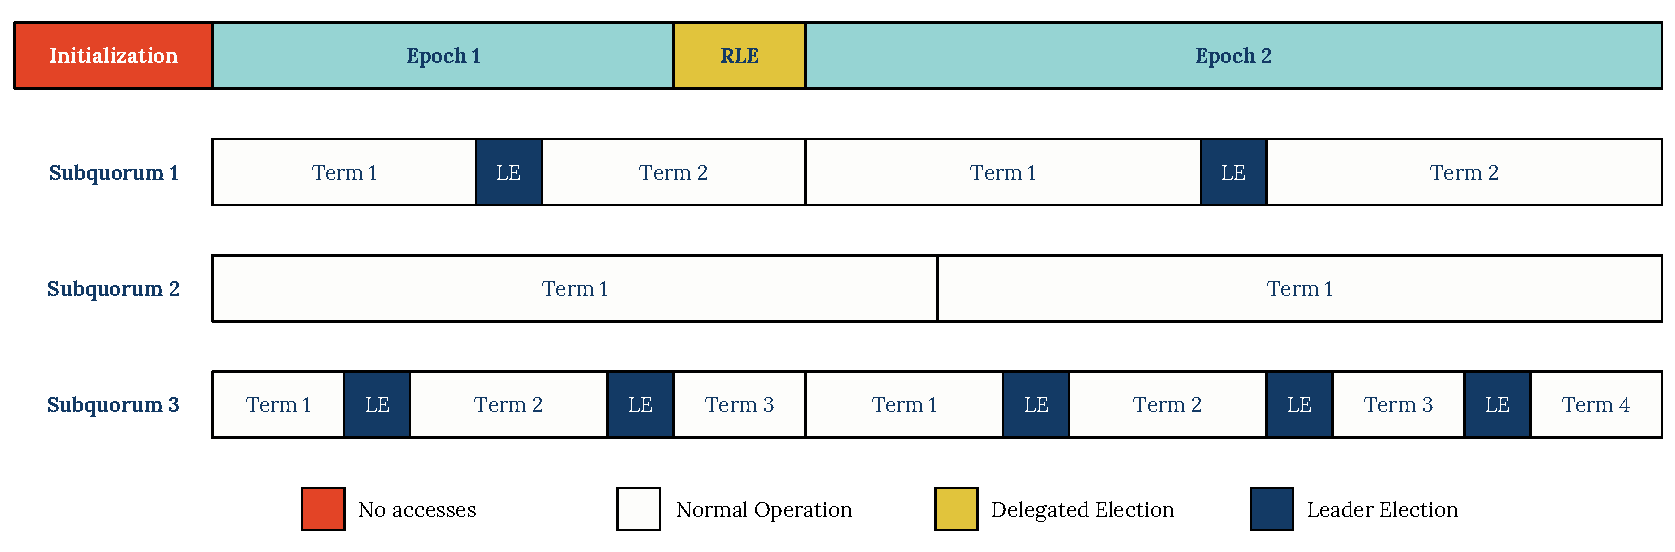
\includegraphics[width=8.2in]{figures/ch03_epochs_terms.pdf}
    \end{center}
    \renewcommand{\baselinestretch}{1}
    \small\normalsize

    \begin{quote}
        \caption[Ordering of Epochs and Terms in Root and Subquorums]{}
        \label{fig:ch03_epochs_terms}
    \end{quote}
\end{figure}
\renewcommand{\baselinestretch}{2}
\small\normalsize
\end{landscape}

\subsection{Fuzzy Handshakes}

Epoch handshakes are required whenever the namespace-to-subquorum mapping changes across an epoch boundary.
HC separates epoch transition announcements in the root quorum from implementation in subquorums.
Epoch transitions are termed \emph{fuzzy} because subquorums need not all transition synchronously.
There are many reasons why a subquorum might be slow.
Communication delays and partitions might delay notification.
Temporary failures might block local commits.
A subquorum might also delay transitioning to allow a local burst of activity to cease such as currently running transactions\renewcommand{\baselinestretch}{1} \small\footnotesize\footnote{The HC implementation discussed in this chapter does not currently support transactions.}\renewcommand{\baselinestretch}{2} \small\normalsize.
Safety is guaranteed by tracking subquorum dependencies across the epoch boundary.

\begin{figure}
    \begin{center}
        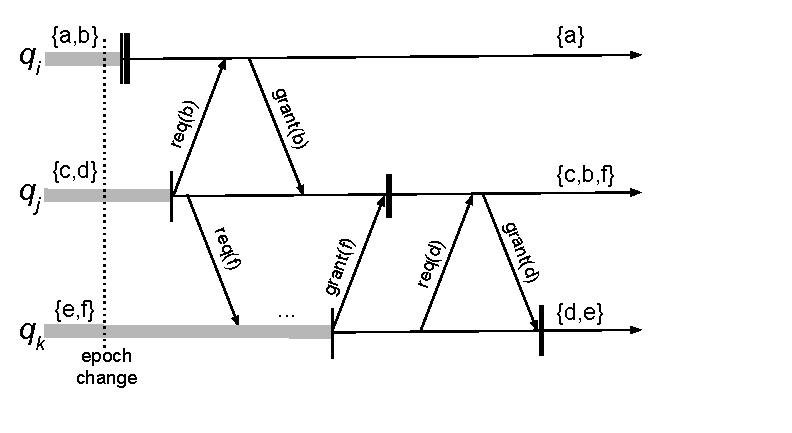
\includegraphics[width=5in]{figures/ch03_namespace_handoff.pdf}
    \end{center}
    \renewcommand{\baselinestretch}{1}
    \small\normalsize

    \begin{quote}
        \caption[Epoch Transition: Fuzzy Handshakes]{Readiness to transition to the new epoch is marked by a thin vertical bar; actual transition is the thick vertical bar.  Thick gray lines indicate operation in the previous epoch.  Subquorum $q_j$ transitions from tag ${c,d}$ to ${c,b,f}$, but begins only after receiving version information from previous owners of those tags.  The request to $q_k$ is only answered once $q_k$ is ready to transition as well.}
        \label{fig:ch03_namespace_handoff}
    \end{quote}
\end{figure}
\renewcommand{\baselinestretch}{2}
\small\normalsize

Figure~\ref{fig:ch03_namespace_handoff} shows an epoch transition where the scopes of $q_i$, $q_j$, and $q_k$ change across the transition as follows:

\todo{Fix the alignment of the below equations:}

\renewcommand{\baselinestretch}{1}
\begin{eqnarray}
    q_{i,x-1} = t_a, t_b  &\longrightarrow q_{i,x} = t_a\\
    q_{j,x-1} = t_c, t_d  &\longrightarrow q_{j,x} = t_c,t_d,t_f\\
    q_{k,x-1} = t_e, t_f  &\longrightarrow q_{k,x} = t_d,t_e
\end{eqnarray}
\renewcommand{\baselinestretch}{2}

All three subquorums learn of the epoch change at the same time, but become ready with varying delays.
These delays could be because of network lags or ongoing local activity.
Subquorum $q_i$ gains no new tags across the transition and moves immediately to the new epoch.
Subquorum $q_j$'s readiness is slower, but then it sends requests to the owners of both the new tags it acquires in the new epoch.
Though $q_i$ responds immediately, $q_k$ delays its response until locally operations conclude.
Once both handshakes are received, $q_j$ moves into the new epoch, and $q_k$ later follows suit.

These bilateral handshakes allow an epoch change to be implemented incrementally, eliminating the need for lockstep synchronization across the entire system.
This flexibility is key to coping with partitions and varying connectivity in the wide area.
However, this piecewise transition, in combination with subquorum re-definition and configuration at epoch changes, also means that individual replicas \emph{may be part of multiple subquorums at a time}.

This overlap is possible because replicas may be mapped to distinct subgroups from one epoch to the next.
Consider $q_k$ in Figure~\ref{fig:ch03_namespace_handoff} again.
Assume the epochs shown are $e_x$ and $e_{x+1}$.
A single replica, $r_a$, may be remapped from subquorum $q_{k,x}$ to subquorum $q_{i,x+1}$ across the transition.
Subquorum $q_{k,x}$ is late to transition, but $q_{i,x+1}$ begins the new epoch almost immediately.
Requiring $r_a$ to participate in a single subquorum at a time would potentially delay $q_{i,x+1}$'s transition and impose artificial synchronicity constraints on the system.
One of the many changes we made in the base Raft protocol is to allow a replica to have multiple distinct shared logs.
Smaller changes concern the mapping of requests and responses to the appropriate consensus group.

\subsection{Subquorum Consensus}

\todo{this section is bad}

Each subquorum, $q_i$, elects a leader to coordinate local decisions.
Fault tolerance of the subquorum is maintained in the usual way, detecting leader failures and electing new leaders from the peers.
Subquorums do not, however, ever change system membership on their own.
Subquorum membership is always defined in the root quorum.

Subquorum consensus is used to commit object writes.
Reads are not committed by default, but are always served by the leader of the
appropriate subquorum.
Namespace assignments in HC result in the object space being partitioned (or
sharded) across distinct subqourms.
The mapping of the shared object namespace to individual subquorums is the
\emph{tagset}, or the tagset partition.
An individual \emph{tag} defines a disjoint subset of the object space.

As writes are committed through HC, the shared logs provide a complete version history of all distributed objects.
Subquorum leaders use in-core caches to provide fast access to recently accessed objects in the local subquorums's tag.
Replicas perform background anti-entropy~\cite{dynamo,bayou,anti_entropy}, disseminating log updates a user-defined number of times across the system.

The most complex portion of the HC protocol is in handling data-related issues at epoch transitions.
Transitions may cause tags to be transferred from one subquorum to another, forcing the new leader to load state remotely to serve object requests.
Transitions handshakes are augmented in three ways.
First, an replica can demand-fetch an object version from any other system replica.
Second, epoch handoffs contain enumerations of all current object versions, though not the data itself.
Knowing an object's current version gives the new handler of a tag the ability to demand fetch an object that is not yet present locally.
Finally, handshakes start immediate fetches of the in-core version cache from the leader of the tag's subquorum in the old epoch to the leader in the new.

We do not currently gather the entire shared log onto a single replica because of capacity and flexibility issues.
Capacity is limited because our system and applications are expected to be long-lived.
Flexibility is a problem because HC, and applications built on HC, gain much of their value from the ability to pivot quickly, whether to deal with changes in the environment or for changing application access patterns.
We require handoffs to be as lightweight as possible to preserve this advantage.

\subsection{Client Operations}

\todo{- Sessions
- Connect to closest available replica, redirected to closest available leader.}

Client namespace accesses are forwarded to the leader of the subquorum for the appropriate part of the namespace.
The underlying Raft semantics ensure that leadership changes do not result in loss of any commits.
Hence, individual- or multiple-client accesses to a single subquorum are totally ordered.
\emph{Remote accesses}, or client accesses to other than their local subquorum, are transparent to the primary protocol.
However, creation of a single shared log of all system operations requires remote accesses to be logged.

\section{Consistency}

Pushing all writes through subquorum commits and serving reads at leaders allows us to guarantee that accesses are linearizable (Lin), which is the strongest non-transactional consistency~\cite{linearizability,sequential_consistency}.
As a recap, linearizability is a combination of atomicity and timeliness guarantees about accesses to a single object.
Both \texttt{reads} and \texttt{writes} must appear atomic, and also instantaneous at some time between a request and the corresponding response to a client.
\texttt{Reads} must always return the latest value.
This implies that reads return values are consistent \emph{with any observed ordering}, i.e., the ordering is \emph{externalizable}~\cite{externalizable}.

Linearizability of object accesses can be \emph{composed}.
If operations on each object are linearizable, the entire object space is also linearizable.
This allows our subquorums to operate independently while providing a globally consistent abstraction.

\subsection{Globally Consistent Logs}
\label{sec:ch03_log_ordering}

Our default use case is in providing linearizable access to an object store.
Though this approach allows us to guarantee all observers will see linearizable results of object accesses in real-time, the system is not able to enumerate a total order, or create a linearizable shared log.
Such a linear order would require fine-grained (expensive) coordination across the entire system, or fine-grained clock synchronization~\cite{spanner}.
Though many or most distributed applications (objects stores, file systems, etc.) will work directly with HC, shared logs are a useful building block for distributed systems.

HC \emph{can} be used to build a sequentially consistent (SC) shared log as shown in Figure~\ref{fig:ch03_log_ordering}.
Like Lin, SC requires all observers to see a single total ordering.
SC differs in that this total ordering does not have to be externalizable.
Instead, it merely has to conform to local operation orders and all reads-from dependencies.

\todo{write about grid consistency}

\begin{landscape}
\begin{figure}
    \begin{center}
        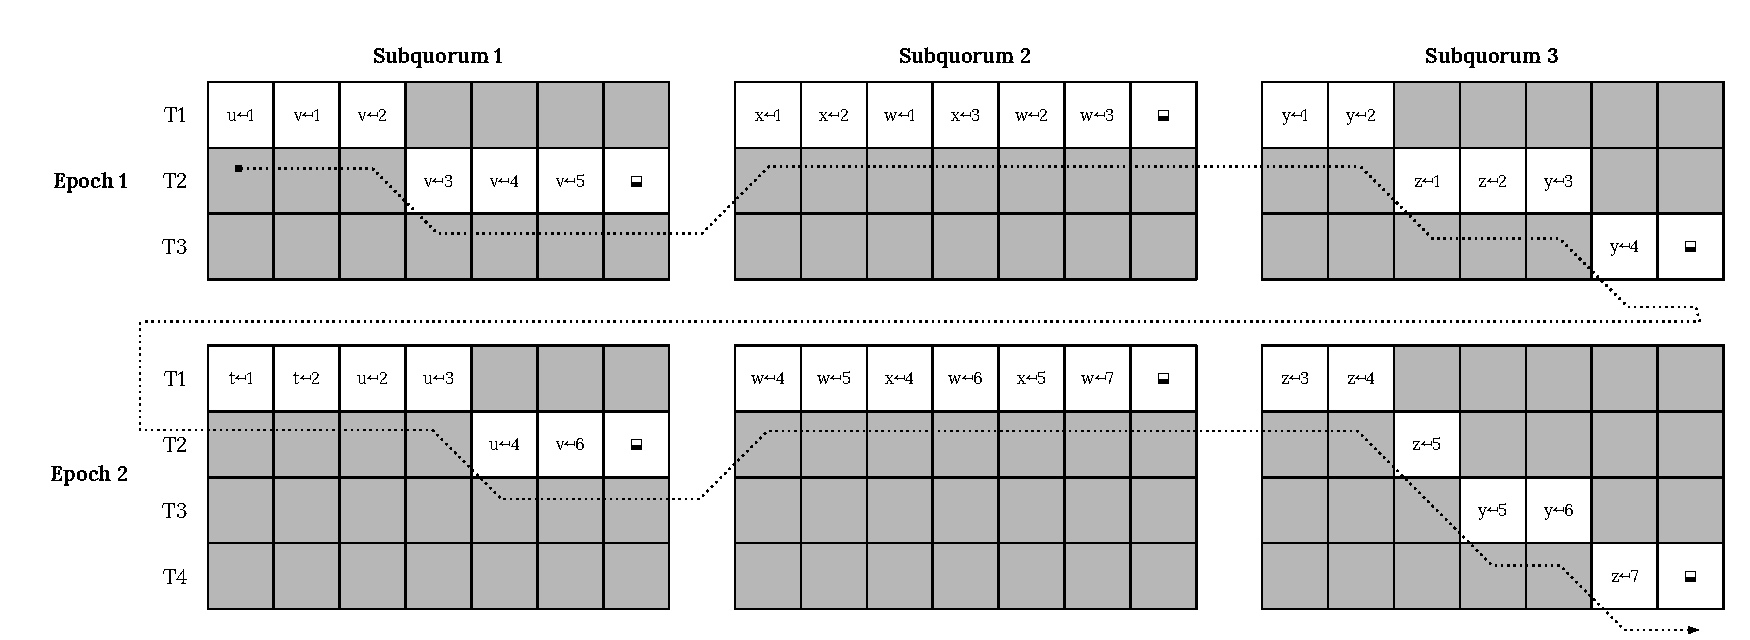
\includegraphics[width=8.2in]{figures/ch03_log_ordering.pdf}
    \end{center}
    \renewcommand{\baselinestretch}{1}
    \small\normalsize

    \begin{quote}
        \caption[Grid Consistency: A Sequential Log Ordering]{}
        \label{fig:ch03_log_ordering}
    \end{quote}
\end{figure}
\renewcommand{\baselinestretch}{2}
\small\normalsize
\end{landscape}


Figure~\ref{fig:ch03_event_ordering} shows a system with subquorums $q_i$ and $q_j$, each of which performs a pair of writes.
Dotted lines show one possible event ordering for replicas $q_i$ (responsible for objects $a$ and $b$), and $q_j$ ($c$ and $d$).
Without cross-subquorum reads or writes, ordering either
subquorums's operations first creates a SC total ordering: $q_i \rightarrow q_j$ (``happened-before''~\cite{lamport_time_1978})
implies $w_{i,1} \rightarrow w_{i,3} \rightarrow w_{j,1} \rightarrow w_{j,3}$,
for example.

\begin{figure}
    \begin{center}
        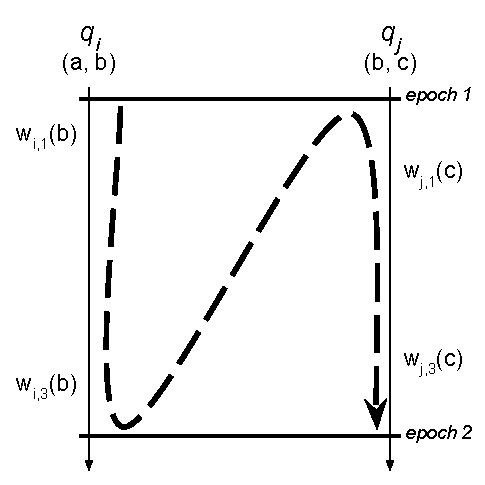
\includegraphics[width=5in]{figures/ch03_event_ordering.pdf}
    \end{center}
    \renewcommand{\baselinestretch}{1}
    \small\normalsize

    \begin{quote}
        \caption[Sequential Event Ordering in HC]{Default ordering: $w_{i,1\rightarrow w_{i,3}\rightarrow w_{j,1}\rightarrow w_{j,3}}$}
        \label{fig:ch03_event_ordering}
    \end{quote}
\end{figure}
\renewcommand{\baselinestretch}{2}
\small\normalsize

By contrast, the subquorums in Figure~\ref{fig:ch03_event_ordering_remote_write} create additional dependencies by issuing remote writes to other subquorums: $w_{i,2} \rightarrow w_{j,3}$ and $w_{j,2} \rightarrow w_{i,3}$.
Each remote write establishes a partial ordering between events of the sender before the sending of the write, and writes by the receiver after the write is received.
Similar dependencies result from remote reads.


\begin{figure}
    \begin{center}
        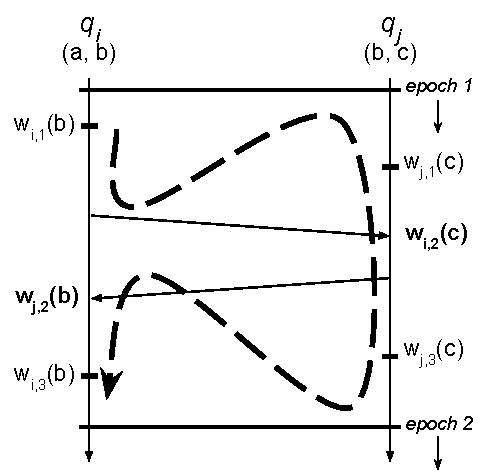
\includegraphics[width=5in]{figures/ch03_event_ordering_remote_write.pdf}
    \end{center}
    \renewcommand{\baselinestretch}{1}
    \small\normalsize

    \begin{quote}
        \caption[Event Ordering with Remote Writes in HC]{Remote writes add additional ordering constraints: $w_{i,1} \rightarrow w_{i,2}\rightarrow w_{j,3}$, and $ w_{j,1} \rightarrow w_{j,2} \rightarrow w_{i,3}$}
        \label{fig:ch03_event_ordering_remote_write}
    \end{quote}
\end{figure}
\renewcommand{\baselinestretch}{2}
\small\normalsize

These dependencies cause the epochs to be split (not shown in picture).
The receipt of write $w_{i,2}$ in $q_j$ causes $q_{j,1}$ to be split into
$q_{j,1.1}$ and $q_{j,1.2}$.
Likewise, the receipt of write $w_{j,2}$ into $q_i$ causes $q_i$ to be split
into $q_{i,1.1}$ and $q_{i,1.2}$.
Any topological sort of the subepochs that respects these orderings, such as
$q_{i,1.1} \rightarrow q_{j,1.1} \rightarrow q_{j,1.2} \rightarrow q_{i,1.2}$,
results in a valid SC ordering.

Presenting a sequentially consistent global log across the entire system, then, only requires tracking these inter-subquorum data accesses, and then performing an $\mathcal{O}(n)$ merge of the subepochs.

By definition, this log's ordering respects any externally visible ordering of cross-subquorum accesses (accesses visible to the system).
However, the log does not necessarily order other accesses according to external visibility.
The resulting shared log could not be mined to find causal relationships between accesses through external communication paths unknown to the system.

For example, assume that log events are published posts, and that one user claimed plagiarism.
The accused would not be able to prove that his post came first unless there were some causal chain of posts and references visible to the protocol.


\section{Fault Tolerance}
\label{sec:fault_tolerance}

We assert that consensus at the leaf replicas is correct and safe because decisions are implemented using well-known leader-oriented consensus approaches.
Hierarchical consensus therefore has to demonstrate linearizable correctness and safety between subquorums for a single epoch and between epochs.
Briefly, linearizability requires external observers to view operations to objects as instantaneous events.
Within an epoch, subquorum leaders serially order local accesses, thereby guaranteeing linearizability for all replicas in that quorum.
% Remote accesses and the internal invariant also enforce linearizability of accesses
% between \subs.

Epoch transitions raise the possibility of portions of the namespace being re-assigned from one subquorum to another, with each subquorum making the transition independently.
Correctness is guaranteed by an invariant requiring subquorums to delay serving newly acquired portions of the namespace until after completing all appropriate handshakes.


\begin{landscape}
\renewcommand{\baselinestretch}{1}
\small\normalsize
 \begin{table}[ht]
\caption[HC Failure Categories]{Failure categories: Peer failure is detected by missed heartbeat messages. The rest are triggered by the appropriate election timeout.}
\begin{center}
\begin{tabular}{l|l}
\hline
Failure Type & Response \\
\hline \hline
subquorum peer & request replica repartition from root quorum \\
subquorum leader & local election, request replacement from root quorum \\
root leader & root election (with delegations)\\
majority of majority of subquorums & (nuclear option) root election after delegations timed out \\
\hline
\end{tabular}
\end{center}
\label{tab:failure_categories}
\end{table}
 \renewcommand{\baselinestretch}{2}
\small\normalsize
\end{landscape}

\subsection{Failures}

During failure-free execution, the root quorum partitions the system into\ disjoint subquorums, assigns \emph{subquorum leaders}, and assigns partitions of the tagspace to subquorums.
Each subquorum coordinates and responds to accesses for objects in its assigned tagspace.
We define the system's \emph{safety} property as guaranteeing that non-linearizable (or non-sequentially-consistent, see Section~\ref{sec:ch03_log_ordering}) event orderings can never be observed.
We define the system's \emph{progress} property as the system having enough live replicas to commit votes or operations in the root quorum.

The system can suffer several types of failures, as shown in Table~\ref{tab:failure_categories}.
Failures of subquorum and root quorum leaders are handled through the normal consensus mechanisms.
Failures of subquorum peers are handled by the local leader petitioning the root quorum to re-configure the subquorum in the next epoch.
Failure of a root quorum peer is the failure of subquorum leader, which is handled as above.
Root quorum heartbeats help inform other replicas of leadership changes, potentially necessary when individual subquorums break down.

\todo{describe assasination}

HC's structure means that some faults are more important than others.
Proper operation of the root quorum requires the majority of replicas in the majority of subquorums to be non-faulty.
Given a system with $2m+1$ subquorums, each of $2n+1$ replicas, the entire system's progress can be halted with as few as $(m+1)(n+1)$ well-chosen failures.
Therefore, in worst case, the system can only tolerate: $f_{worst}=mn+m+n$ failures and still make progress.
At maximum, HC's basic protocol can tolerate up to: $f_{best} = (m+1)*n + m*(2n+1) = 3mn+m+n$ failures.
As an example, a 25/5 system can tolerate at least 8 and up to 16 failures out of 25 total replicas.
A 21/3 system can tolerate at least 7, and a maximum of 12, failures out of 21 total replicas.
Individual subquorums might still be able to perform local operations despite an impasse at the global level.

Total subquorum failure can temporarily cause a portion of the namespace to be unserved.
However, the root quorum eventually times out and moves into a new epoch with that portion assigned to another subquorum.

\subsection{Obligations Timeout}

\todo{write this section}

\subsection{The Nuclear Option}
\label{sec:nuclear}

\todo{fix this section}

Singleton consensus protocols, including Raft, can tolerate just under half of the entire system failing.
As described above, HC's structure makes it more vulnerable to clustered failures.
Therefore we define a \emph{nuclear option}, which uses direct consensus decision among all system replicas to tolerate any $f$ replicas failing out of $2f+1$ total replicas in the system.

A nuclear vote is triggered by the failure of a root leader election.
A \emph{nuclear candidate} increment's its term for the root quorum and broadcasts a request for votes to all system replicas.
The key difficulty is in preventing delegated votes and nuclear votes from reaching conflicting decisions.
Such situations might occur when temporarily unavailable subquorum leaders regain connectivity and allow a wedged root quorum to unblock.
Meanwhile, a nuclear vote might be concurrently underway.

Replica delegations are defined as intervals over specific slots.
Using local subquorum slots would fall prey to the above problem, so we define delegations as a small number (often one) of root slots, which usually correspond to distinct epochs.
During failure-free operation, peers delegate to their leaders and are all represented in the next root election or commit.
Peers then renew their delegations to their leaders by appending them to the next local commit reply.
This approach works for replicas that change subquorums over an epoch boundary, and even allows peers to delegate their votes to arbitrary other peers in the system (see replicas $r_N$ and $r_O$ in Figure~\ref{fig:ch03_tiers}).

This approach is simple and correct, but deals poorly with leader turnovers in the subquorum.
Consider a subquorum where all peers have delegated votes to their leader for the next root slot.
If that leader fails, none of the peers will be represented.
We finesse this issue by re-defining such delegations to count root elections, root commits, \emph{and} root heartbeats.
The latter means that local peers will regain their votes for the next root quorum action if it happens after to the next heartbeat.

Consider the worst-case failure situation discussed in Section~\ref{sec:fault_tolerance}: a majority of the majority of subquorums have failed.
None of the failed subquorum leaders can be replaced, as none of those subquorums have enough local peers.

The first response is initiated when a replica holding delegations (or its own vote) times out waiting for the root heartbeat.
That replica increments its own root term, adopts the prior system configuration as its own, and becomes a root candidate.
This candidacy fails, as a majority of subquorum leaders, with all of their delegated votes, are gone.
Progress is not made until delegations time out.
In our default case where a delegation is for a single root event, this happens after the first root election failure.

At the next timeout, any replica might become a candidate because delegations have lapsed (under our default assumptions above).
Such a \emph{nuclear} candidate increments its root term and sends candidate requests to all system replicas, succeeding if it gathers a majority across all live replicas.

The first candidacy assumed the prior system configuration in its candidacy announcement.
This configuration is no longer appropriate unless some of the ``failed'' replicas quickly regain connectivity.
Before the replica announces its candidacy for a second time, however, many of the replica replies have timed out.
The candidate alters its second proposed configuration by recasting all such replicas as hot spares and potentially reducing the number and size of the subgroups.
Subsequent epoch changes might re-integrate the new hot spares if the replicas regain connectivity.

\section{Performance Evaluation}
\label{sec:evaluation}

HC was designed to adapt both to dynamic workloads as well as variable network conditions.
We therefore evaluate HC in two distinct environments: a homogeneous data center and a heterogeneous real-world network.
The homogeneous cluster is hosted on Amazon EC2 and includes 26 ``t2.medium'' instances: dual-core virtual machines running in a single VPC with inter-machine latencies of $\lambda_{\mu}=0.399ms$ and $\lambda_{\sigma}=0.216ms$.
These machines are cost effective and, though lightweight, are easy to scale to large cluster sizes as workload increases.
Experiments are set up such that each instance runs a single replica process and multiple client processes.

The heterogeneous cluster (UMD) consists of several local machines distributed across a wide area, with inter-machine latencies ranging from
$\lambda_{\mu}=2.527ms$,
$\lambda_{\sigma}=1.147ms$ to $\lambda_{\mu}=34.651ms$,
$\lambda_{\sigma}=37.915ms$.
Machines in this network are a variety of dual and quad core desktop servers that are solely dedicated to running these benchmarks.
Experiments on these machines are set up so that each instance runs multiple replica and client processes co-located on the same host.
In this environment, localization is critical both for performance but also to ensure that the protocol can elect and maintain consensus leadership.
The variability of this network also poses challenges that HC is uniquely suited to handle via root quorum-guided adaptation.
We explore two distinct scenarios -- sawtooth and repartitioning -- using this cluster; all other experiments were run on the EC2 cluster.

\begin{figure}
    \begin{center}
        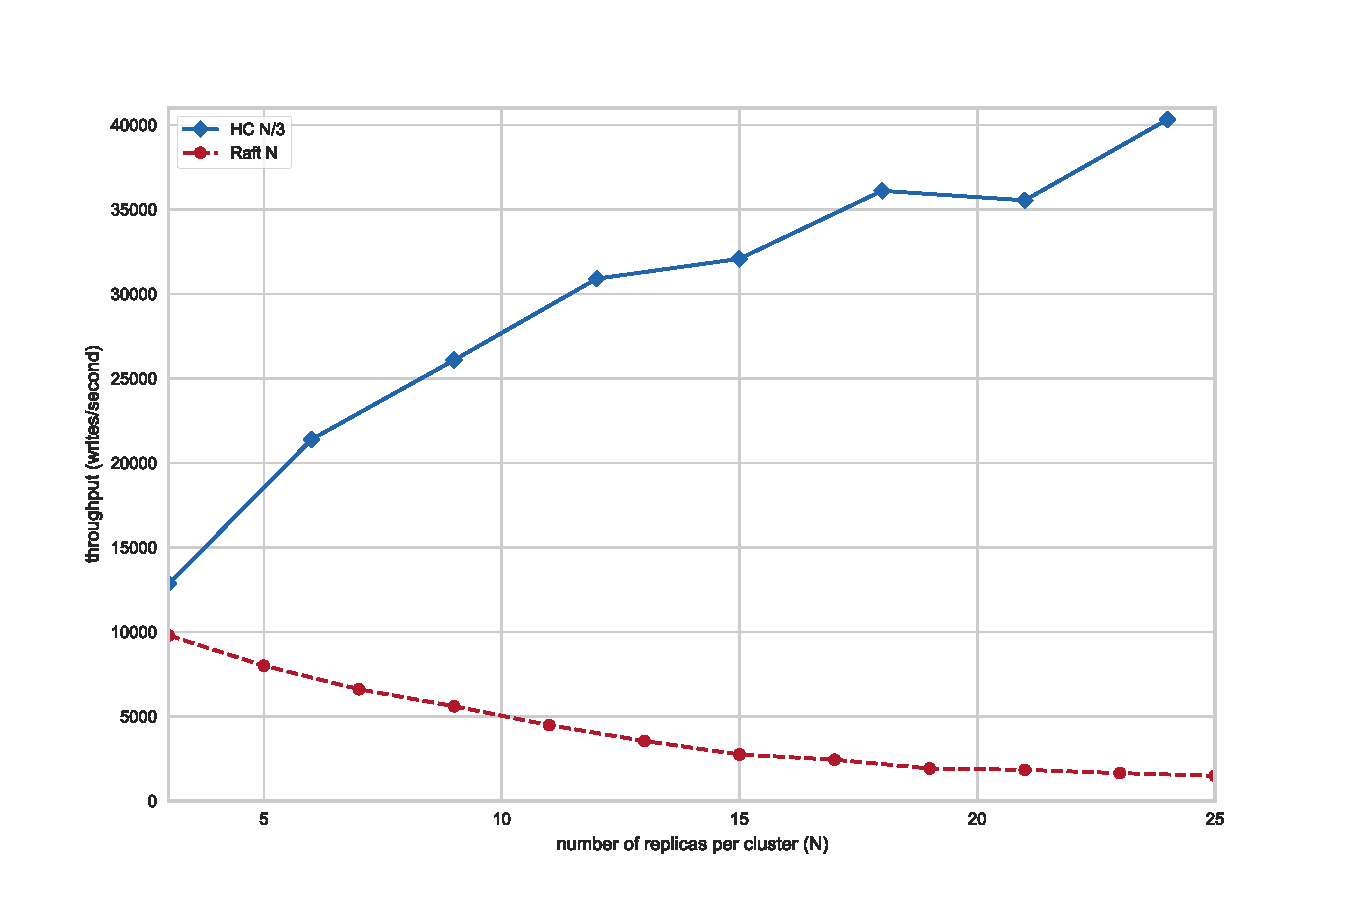
\includegraphics[width=5in]{figures/ch03_scaling_consensus.pdf}
    \end{center}
    \renewcommand{\baselinestretch}{1}
    \small\normalsize

    \begin{quote}
        \caption[Scaling Consensus HC vs. Raft]{Mean throughput of workloads of up to 120 concurrent clients}
        \label{fig:ch03_scaling_consensus}
    \end{quote}
\end{figure}
\renewcommand{\baselinestretch}{2}
\small\normalsize

HC is partially motivated by the need to scale strong consistency to large cluster sizes.
We based our work on the assumption that consensus performance decreases as the quorum size increases, which we confirm empirically in Figure~\ref{fig:ch03_scaling_consensus}.
This figure shows the maximum throughput against system size for a variety of workloads, up to 120 concurrent clients.
A workload consists of one or more clients continuously sending writes of a specific object or objects to the cluster without pause.

Standard consensus algorithms, Raft in particular, scale poorly with uniformly decreasing throughput as nodes are added to the cluster.
Commit latency increases with quorum size as the system has to wait for more responses from peers, thereby decreasing overall throughput.
Figures~\ref{fig:ch03_scaling_consensus} and~\ref{fig:ch03_hc_throughput_workload} clearly show the multiplicative advantage of HC's hierarchical structure, though HC does not scale linearly as we had expected.

\begin{figure}
    \begin{center}
        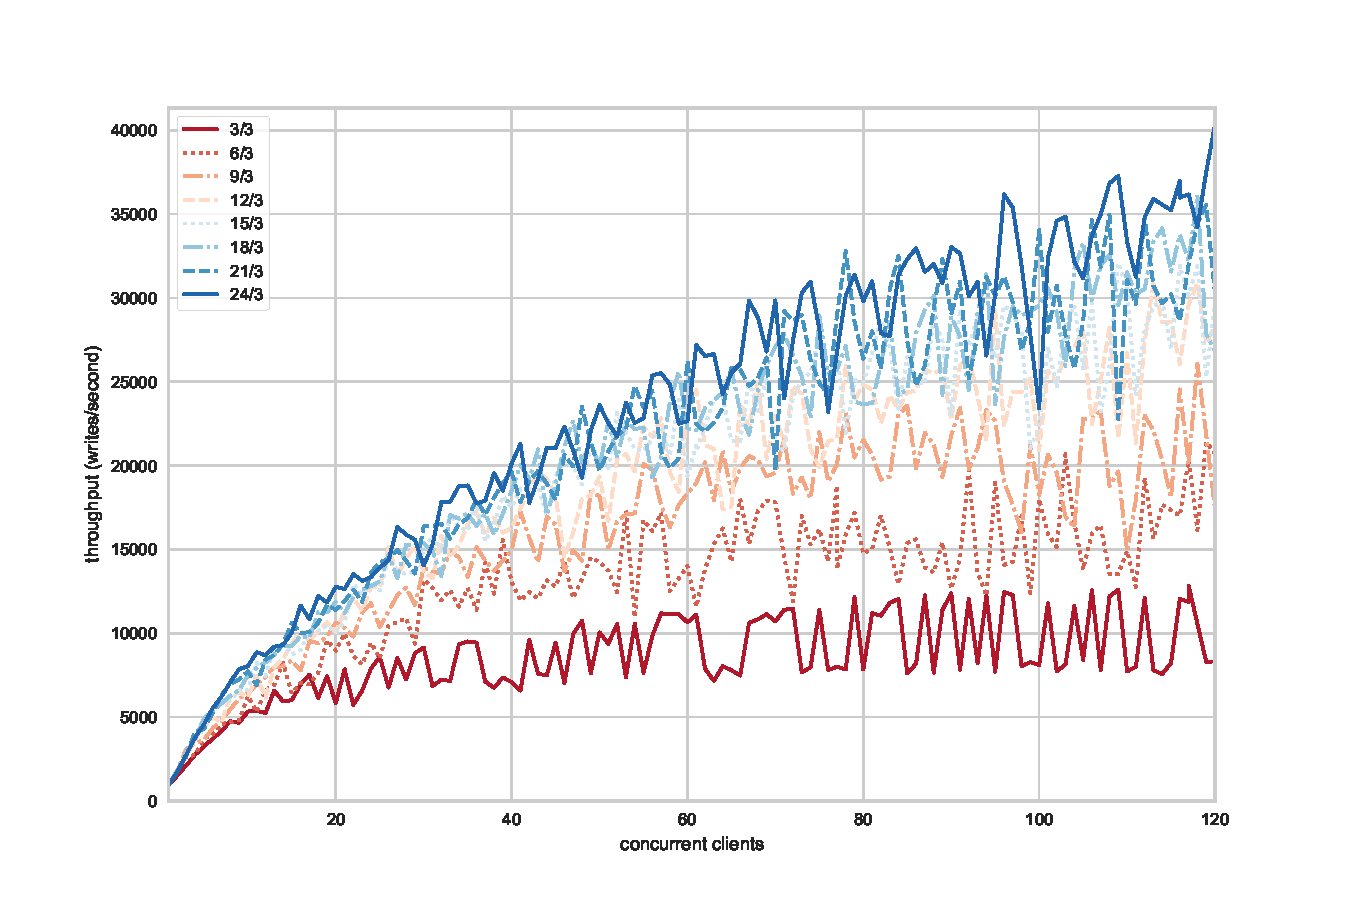
\includegraphics[width=5in]{figures/ch03_hc_throughput_workload.pdf}
    \end{center}
    \renewcommand{\baselinestretch}{1}
    \small\normalsize

    \begin{quote}
        \caption[HC Throughput vs. Workload in the Wide Area]{Performance of distributed consensus with an increasing workload of concurrent clients. Performance is measured by throughput, the number of writes committed per second.}
        \label{fig:ch03_hc_throughput_workload}
    \end{quote}
\end{figure}
\renewcommand{\baselinestretch}{2}
\small\normalsize

There are at least two factors currently limiting the HC throughput shown here.
First, the HC subquorums for the larger system sizes are not saturated.
A single 3-node subquorum saturates at around 25 clients and this experiment has only about 15 clients per subquorum for the largest cluster size.
We ran experiments with 600 clients, saturating all subquorums even in the 24-node case.
This throughput peaked at slightly over 50,000 committed writes per second, better but still lower than the linear scaling we had expected.

We think the reason for this ceiling is hinted at by Figure~\ref{fig:ch03_hc_throughput_workload}.
This figure shows increasingly larger variability with increasing system sizes.
A more thorough examination of the data shows widely varying performance across individual subquorums in the larger configurations.
We suspect that the cause is either VM misconfiguration or misbehavior.
We are adding more instrumentation to diagnose the problem.

\begin{figure}
    \begin{center}
        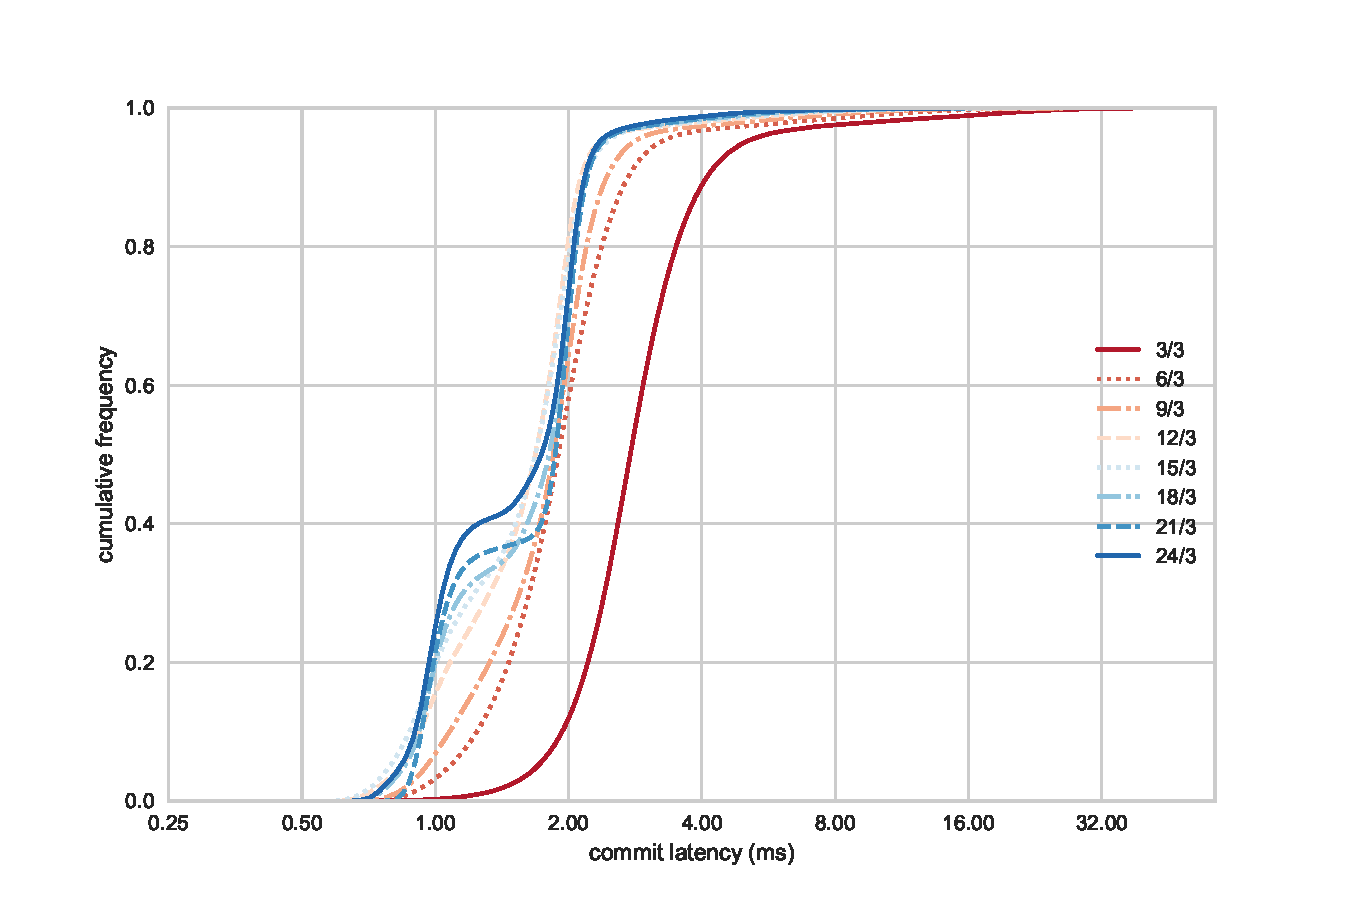
\includegraphics[width=5in]{figures/ch03_ec2_latency_cumfreq.pdf}
    \end{center}
    \renewcommand{\baselinestretch}{1}
    \small\normalsize

    \begin{quote}
        \caption[HC Cumulative Latency Distribution]{}
        \label{fig:ch03_ec2_latency_cumfreq}
    \end{quote}
\end{figure}
\renewcommand{\baselinestretch}{2}
\small\normalsize

The effect of saturation is also demonstrated in Figure~\ref{fig:ch03_ec2_latency_cumfreq}, which shows cumulative latency distributions for different system sizes holding the  workload (number of concurrent clients) constant.
The fastest (24/3) shows nearly 80\% of client write requests being serviced in under 2 msec.
Larger system sizes are faster because the smaller systems suffer from contention (25 clients can saturate a single subquorum).
Because throughput is directly related to commit latency, throughput variability can be mitigated by adding additional subquorums to balance load.

Besides pure performance and scaling, HC is also motivated by the need to adapt to varying environmental conditions.
In the next set of experiments, we explore two common runtime scenarios that motivate adaptation: shifting client workloads and failures.
We show that HC is able to adapt and recover with little loss in performance. These scenarios are shown in Figures~\ref{fig:ch03_umd_sawtooth} and \ref{fig:ch03_umd_fault_tolerance} as throughput over time, where vertical dotted lines indicate an epoch change.

\begin{figure}
    \begin{center}
        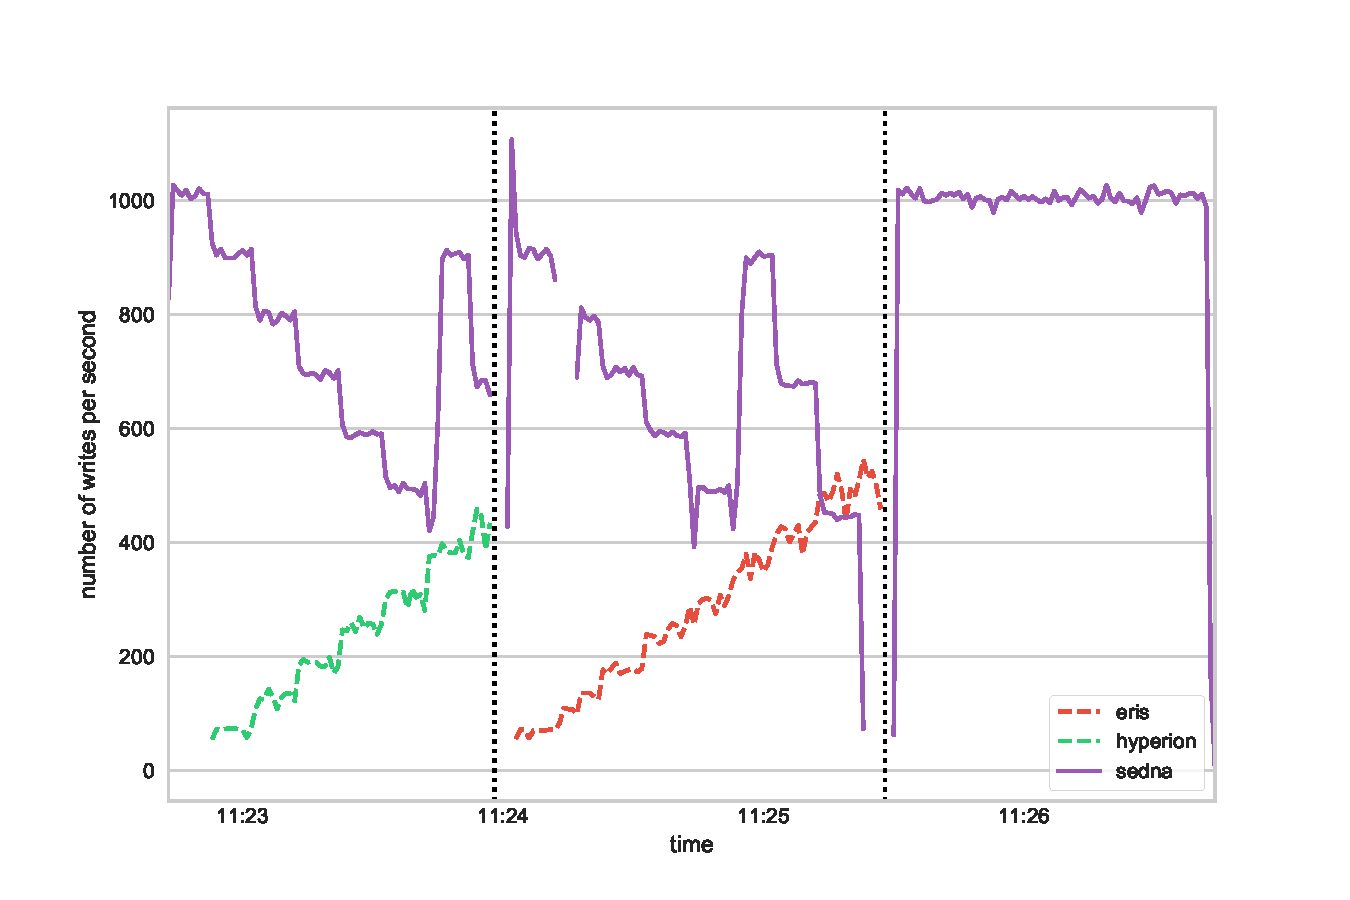
\includegraphics[width=5in]{figures/ch03_umd_sawtooth.pdf}
    \end{center}
    \renewcommand{\baselinestretch}{1}
    \small\normalsize

    \begin{quote}
        \caption[Sawtooth Graph]{9/3 system adapting to changing client access patterns by repartitioning the tag space so that clients are co-located with subquorums that serve tags they need.}
        \label{fig:ch03_umd_sawtooth}
    \end{quote}
\end{figure}
\renewcommand{\baselinestretch}{2}
\small\normalsize

The first scenario, described by the time series in Figure~\ref{fig:ch03_umd_sawtooth} shows an HC 3-replica configuration moving through two epoch changes.
Each epoch change is triggered by the need to localize tags accessed by
clients to nearby subquorums.
% The experiment was run over machines with widely varying latency.
The scenario shown starts with all clients co-located with the subquorum serving the tag they are accessing.
However, clients incrementally change their access patterns first to a tag located on one remote subquorum, and then to the tag owned by the other.
In both cases, the root quorum adapts the system by repartitioning the tagspace such that the tag defining their current focus is served by the co-located subquorum.

\begin{figure}
    \begin{center}
        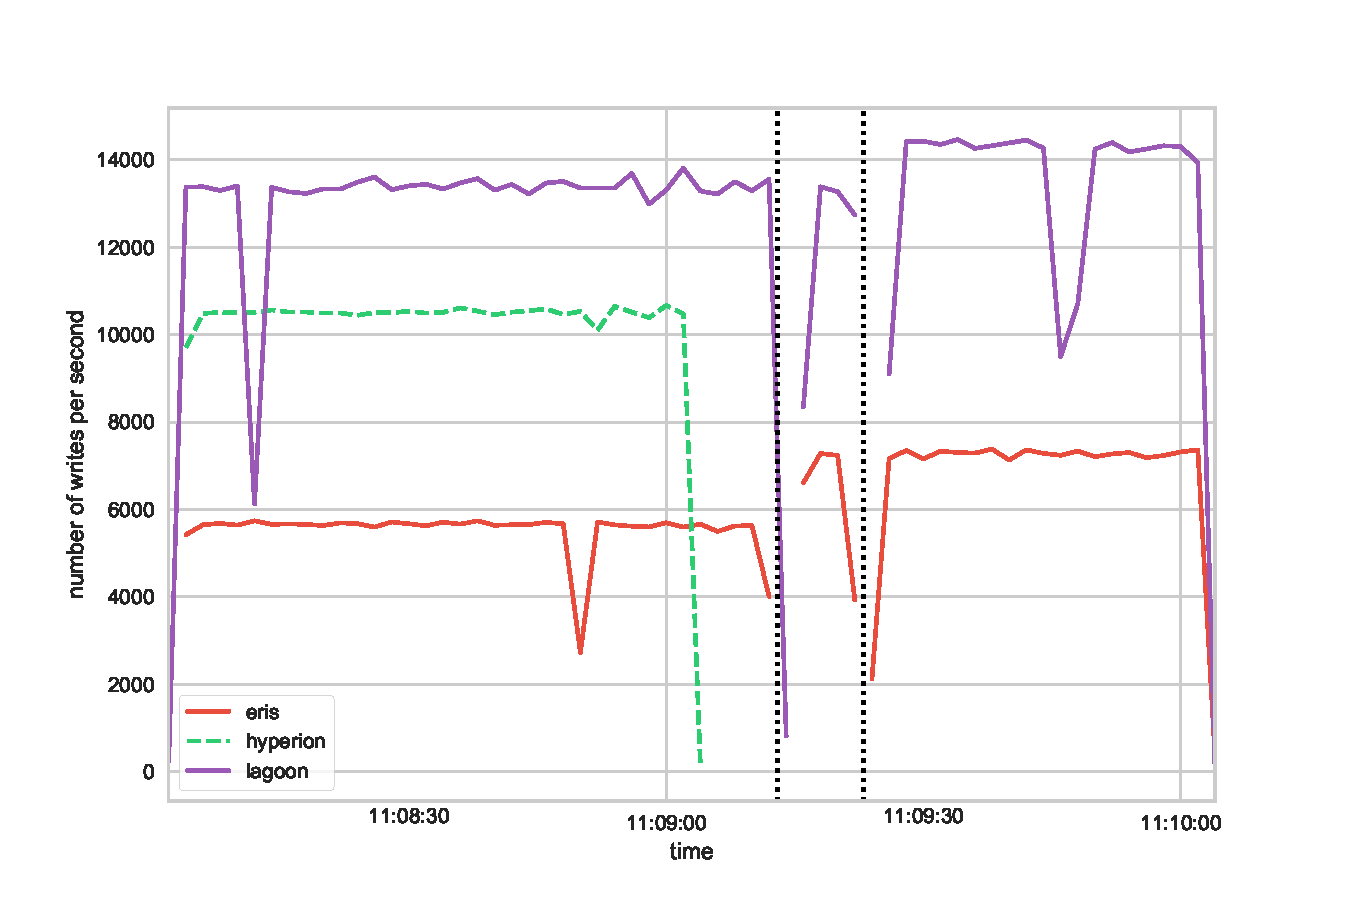
\includegraphics[width=5in]{figures/ch03_umd_fault_tolerance.pdf}
    \end{center}
    \renewcommand{\baselinestretch}{1}
    \small\normalsize

    \begin{quote}
        \caption[HC Fault Repartitioning]{9/3 System that adapts to failure (partition) of entire subquorum. After timeout, the root quorum re-partitions the tag allocated to the failed subquorum among the other two subquorums.}
        \label{fig:ch03_umd_fault_tolerance}
    \end{quote}
\end{figure}
\renewcommand{\baselinestretch}{2}
\small\normalsize

Finally, Figure~\ref{fig:ch03_umd_fault_tolerance} shows a 3-subquorum configuration where one entire subquorum becomes partitioned from the others.
After a timeout, the root uses an epoch change to re-allocate the tag of the partitioned subquorum over the two remaining subquorums.
The partitioned subquorum eventually has an \emph{obligation timeout}, after which the root quorum is not obliged to leave the tag with the current subquorum.
The tag may then be re-assigned to any other subquorum.
Timeouts are structured such that by the time an obligation timeout fires, the root quorum has already re-mapped that subquorum's tag to other subquorums.
As a result, the system is able to recover from the partition as fast as possible.
Note that in this figure, the repartition occurs through two epoch changes, the first allocating part of the tagspace to the first subquorum, and the second allocating the rest of the tag to the other.
Gaps in the graph are periods where the subquorums are electing local leaders.
This may be optimized by having leadership assigned or maintained through root consensus.

\section{Conclusion}

Most consensus algorithms have their roots in the Paxos algorithm, originally described in parliamentary terms.
The metaphor of government still applies well as we look at the evolution of distributed coordination as systems have grown to include large numbers of processes and geographies.
Systems that use a dedicated leader are easy to reason about and implement, however, like chess, if the leader goes down the system cannot make any\ progress.
Simple democracies for small groups solve this problem but do not scale, and as the system grows, it fragments into tribes.
Inspired by modern governments, we have proposed a representative system of consensus, hierarchical consensus, such that replicas elect leaders to participate in a root quorum that makes decisions about the global state of the system.
Local decision making, the kind that effects only a subset of clients and objects is handled locally by subquorums as efficiently as possible.
The result is a a hierarchy of decision making that takes advantage of hierarchies that already exist in applications.

Hierarchical Consensus is an implementation and extension of Vertical Paxos.
Like Vertical Paxos, HC reasons about consistency across all objects by identifying commands with a grid ordering (rather than a log ordering) and is reconfigurable to adapt to dynamic environments that exist in geo-replicated systems.
Adaptability allows HC to exploit locality of access, allowing for high performance coordination, even with replication across the wide area.
HC extends Vertical Paxos to ensure that intersections exist between the subquorums and the root quorum to ensure coordination exists between subquorums and to ensure that the system operates as a coordinated whole.
To scale the consensus protocol of the root quorum, we propose a novel approach, delegation, to ensure that all replicas participate in consensus but limit the number and frequency of messages required to achieve majority.
Finally, we generalized HC from primary-backup replication to describe more general online replication required by distributed databases and file systems.

In the next chapter we'll explore a hybrid consistency model implemented by federating replicas that participate in different consistency protocols.
In a planetary scale network, HC provides the strong consistency backbone of the federated model, increasing the overall consistency of the system by making coordinating decisions at a high level, and allowing high availability replicas in the fog operate independently where necessary.
